%
% 
%
\let\textcircled=\pgftextcircled
\chapter{Real Space Analysis of Active Colloids in a 3D Complex Environment}
\label{chap:expSystem}

\initial{I}n this chapter we present the first three-dimensional active colloidal system in non-trivial confinement. The system is comprised of active Janus particles driven via an external field, propelling through the porous network surrounding a colloidal gel. This system is imaged in real-time with confocal microscopy and the particle dynamics are extracted with particle tracking methods. Herein, we will detail the reproducible methodology used to assemble this system, and present and discuss results to date. 




\section{Introduction}


As mentioned previously, the transport of organic active matter occurs naturally in complex environments such as porous soils \cite{gannon1991} and organic tissues \cite{isermann2017}.
These real-life biological active systems are highly complex and feature many overlapping interactions that make comparison with theoretical predictions difficult. To address this issue, many model systems have been designed to study active matter in situations wherein the interactions between the active units and their environment are largely understood. One popular experimental  system for modelling the physics of active matter on mesoscopic lengthscales is colloids \cite{vernerey2019}. These particles benefit from their size, as they are subject to the same Brownian motion as organic examples of active matter  (such as bacteria \cite{purcell2016}). 
 Furthermore, colloids are highly versatile and can be functionalised to possess a wide range of particle interactions \cite{zhang2017, pawar2010}, or be engineered to exhibit certain behaviours such as self-propulsion \cite{ebbens2016}. 
 
 With the growing interest in active systems, there have been several studies of colloids in artificial patterned landscapes; seeking to understand the physics governing the dynamics of active bodies in heterogeneous environments. For example, active colloids can undergo smooth transitions from diffusive, to subdiffusive, to localisation with an increase in the density of environmental obstacles \cite{morin2017}, in agreement with computational models \cite{zeitz2017,reichhardt2014}. Furthermore, populations of active colloids exhibit clogging phenomena on disordered landscapes, where collisions with obstacles result in localised arrest \cite{stoop2018, leyva2020}, and these effects are enhanced at higher particle speeds. Moreover, above threshold densities the clogging of colloids can induce a jammed state, where the individual particles compact into a solid-like phase with finite yield \cite{cates1998,stoop2018,lips2021}.

 
 All of the systems mentioned above are quasi-2D systems, i.e. active particles  moving across a 2D landscape. However, without information regarding the dynamics of active systems in three-dimensions, we are limited as to what we can understand of real-life biological systems. One notable exception \cite{bhattacharjee2019} observed a bacterium microswimmer in a 3D porous environment. Herein, the environmental constriction was found to inhibit the reorientation mechanism, leading to long persistent paths directed by the environment. 
In the previous chapters, we have seen the importance of dimensionality in simulations of spherical active systems; in this chapter we extend this idea to experimental systems. Here we create an experimental system in which active colloids undergo motion similar to active Brownian motion within a three-dimensional porous environment. The active colloids in this work are Janus particles which perform self-phoretic motion in the presence of an external electric field, and the complex environment within which they inhabit is the random, branching structure of a colloidal gel. 

\begin{figure*}
	\centering
	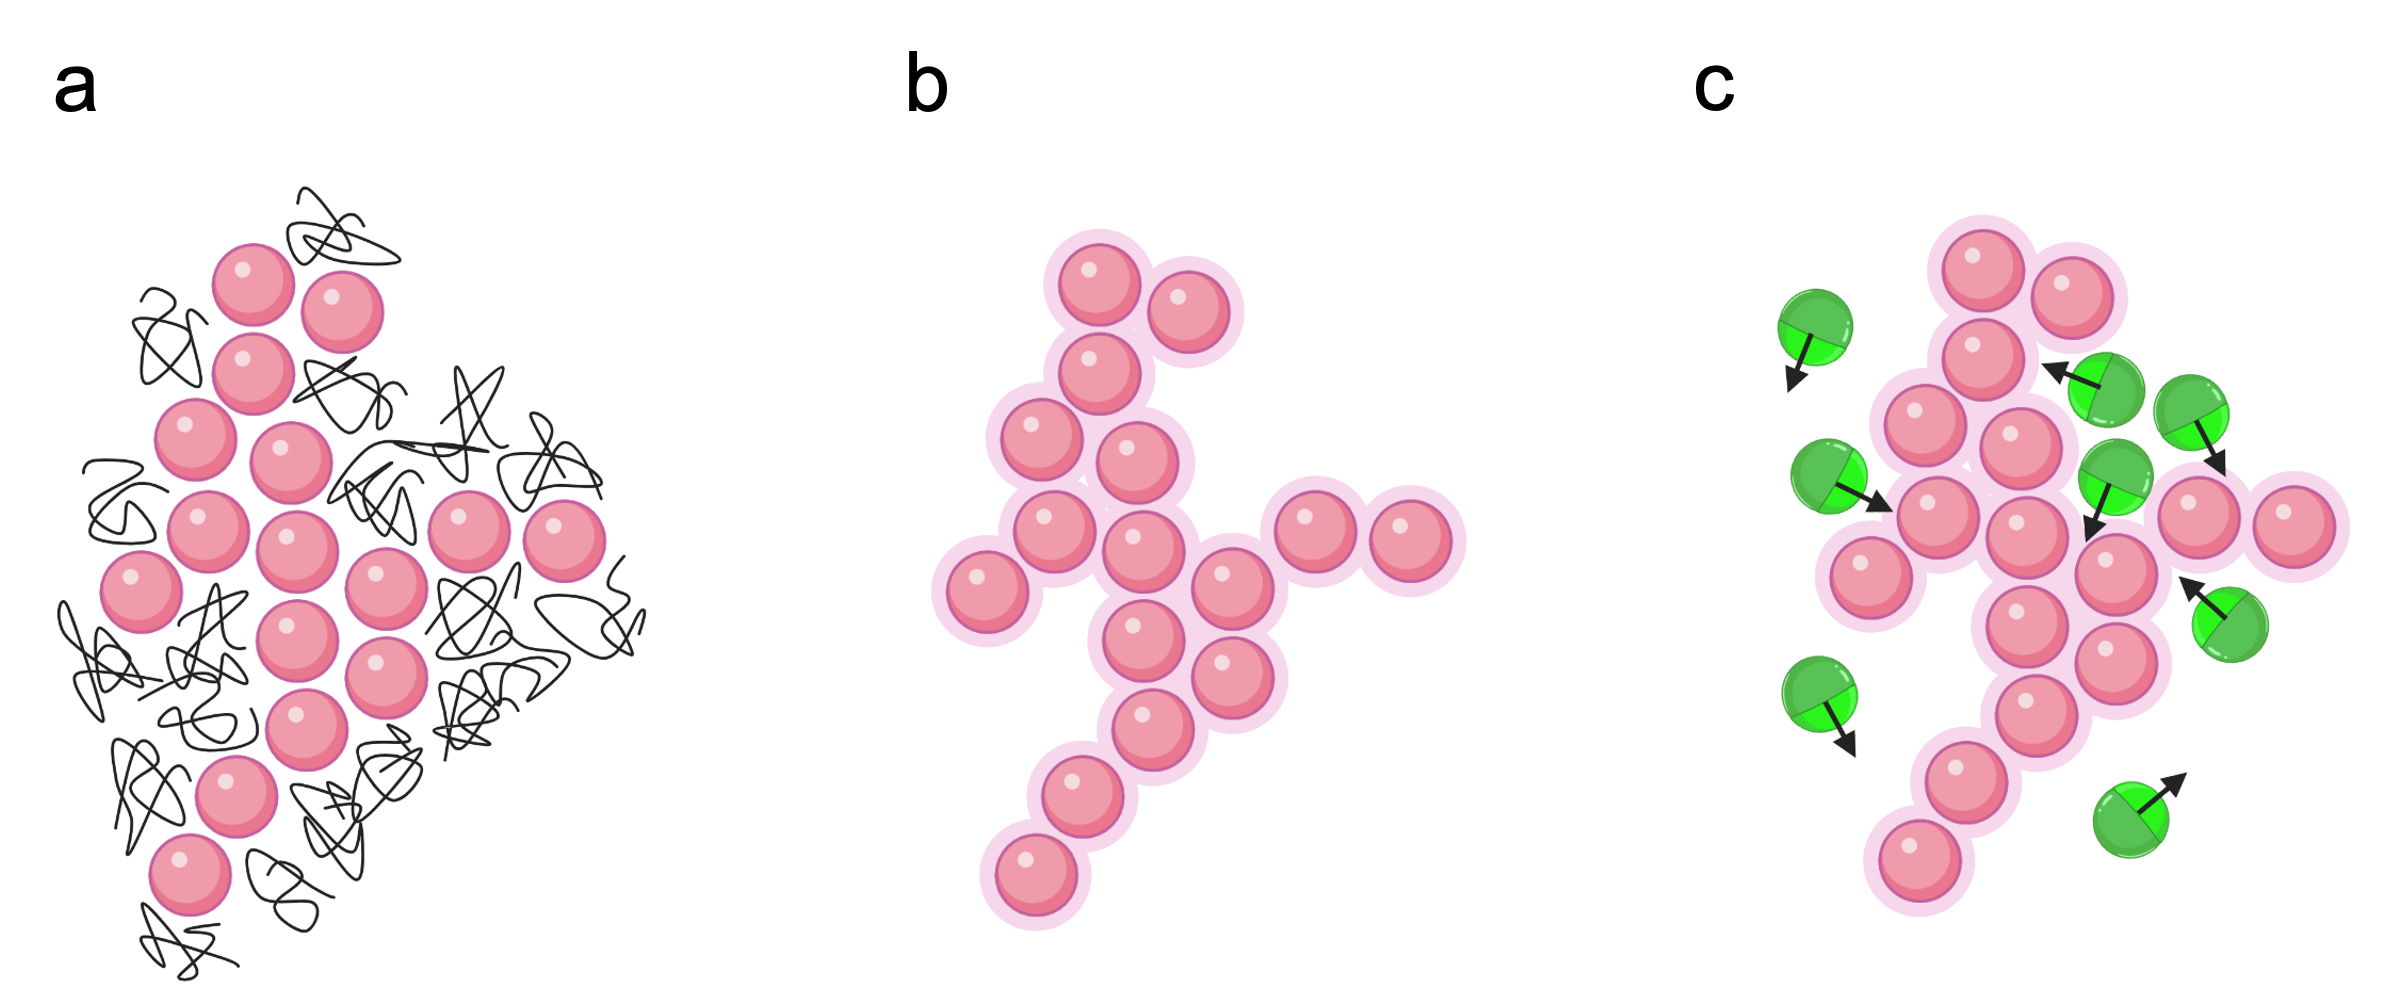
\includegraphics[width=\linewidth]{figsExpSystem/figSummary}
	\caption[Schematic depicting the three step process used to assemble the experimental 3D active system]{Schematic depicting the three step process used to assemble the 3D active system used in this work: \textbf{a} Colloids (pink) are assembled into a gel with the addition of a non-adsorbing polymer (black). \textbf{b} A thin shell is grown around the gel network joining the colloids together, after which the polymer is removed. \textbf{c} Active Janus colloids (green)  are inserted into the vacant spaces around the gel and the active dynamics imaged are by confocal microscopy. }
	\label{fig:ExpSummary}
\end{figure*}


To achieve the realisation of a 3D active colloidal system within a non-trivial heterogeneous environment; active Janus particles and colloidal gels are brought together through a three-step process (summarised in Fig. \ref{fig:ExpSummary}). The first step regards the creation of a colloidal gel that will provide the structure of the complex environment. This gel is assembled with a colloid-polymer mixture (Fig. \ref{fig:ExpSummary}a). Following this, the gel goes through a \textit{sintering} process, where the colloids are physically joined together through the growth of a solid material shell that encompasses the network (Fig. \ref{fig:ExpSummary}b). 
The purpose of this step is to replace the mechanism responsible for maintaining the structure of the gel, as the presence of the polymer (which is dispersed through the solvent surrounding the colloids), will not allow for the free motion of Janus particles.
With the gel sintered, the polymer can subsequently be removed, after which a suspension of Janus particles is added to the sample.  These Janus particles are dispersed throughout the pores surrounding the colloidal gel network, through which they undergo active motion upon the application of an external electric field (Fig. \ref{fig:ExpSummary}c).

The active Janus particles featured in this thesis achieve self-propulsion via induced-charge electrophoresis (ICEP) \cite{gangwal2008,nishiguchi2015,yan2016,vanderlinden2019}. When exposed to an external electric field from two parallel electrodes, these Janus particles experience a torque aligning the particle equators with the field lines. If the electric field acts in the $z$ plane, the induced asymmetric ionic flow around the particles causes it to propel in a manner alike to that of active Brownian motion in the $xy$ plane. In the $z$ direction the particles exhibit diffusive Brownian motion only.
These ICEP dynamics are sensitive to the electric field strength and the frequency of the electric field. A previous work \cite{sakai2020} with these particles in the bulk found that in the dilute regime, the particles behave analogously to active Brownian particles at low field strength.

This chapter is structured as follows: In section \ref{section:expSystem:Methods}, we describe in detail the methodology used to assemble this experimental system and the process through which the observation of active dynamics is observed in said system. Within section \ref{section:expSystem:Results}, a series of results to date are presented demonstrating the capabilities of this system, along with a discussion of phenomena observed. Finally, this chapter concludes in section \ref{section:expSystem:Conclusion} with a summary of the findings contained in this work, along with a discussion of possible continuations within this area.




\section{Methods}
\label{section:expSystem:Methods}

In the following section we will outline in detail the process for assembling the system depicted in Fig. \ref{fig:ExpSummary}. The assembly for this system  has several stages, and we have therefore broken the process down into multiple sections: First, we detail the design and assembly of the electrical microfluidic sample cell which will house the gel and the Janus particles. Following this, the steps for the assembly of the colloidal gel within the microfluidic system are outlined along with the process of sintering the gel network. Finally, the methodology for the insertion of the Janus particles into the gel is detailed, and followed by an instructive breakdown for the assembly of the electrical apparatus used during the microscopy of active dynamics.

\subsection{Sample cell}
\label{section:SampleCell}

The cell that holds the sample must satisfy several requirements: The cell must have an inlet and an outlet for the microfluidic tubing; the top and bottom walls of the cell must be conductive to allow for connection to a circuit; such that an ac field can be generated. Finally, the top wall of the cell must be both optically transparent and sufficiently thin ($<100\mu$m) to allow for high quality microscopy of the sample. 


A schematic of the sample cell is shown in Fig. \ref{fig:SampleCell}. In the  top view of the figure, the location of the sample chamber is highlighted with a dotted line. This is the where the gel will be assembled and where the dynamics of the Janus particles will be imaged. The sample chamber is enclosed on all sides. Above and below, the chamber is bordered by thin glass planes coated in Indium Tin Oxide (ITO) a widely used transparent conductive oxide (\textit{SPI Supplies: thickness 0.13-0.17mm, resistivity 70 - 100 ohms}), to which the wires leading to the signal generator will connect. Two opposing sides are formed from cut glass slides of identical thickness to that of the slide forming the base, these are used to obtain a well defined height for the chamber, sufficient for the tubing. Plastic tubing forms the final two opposing boundaries to the sample chamber, each with a narrow channel that is used to form the inlet and outlet to the chamber. 

\begin{figure*}
	\centering
	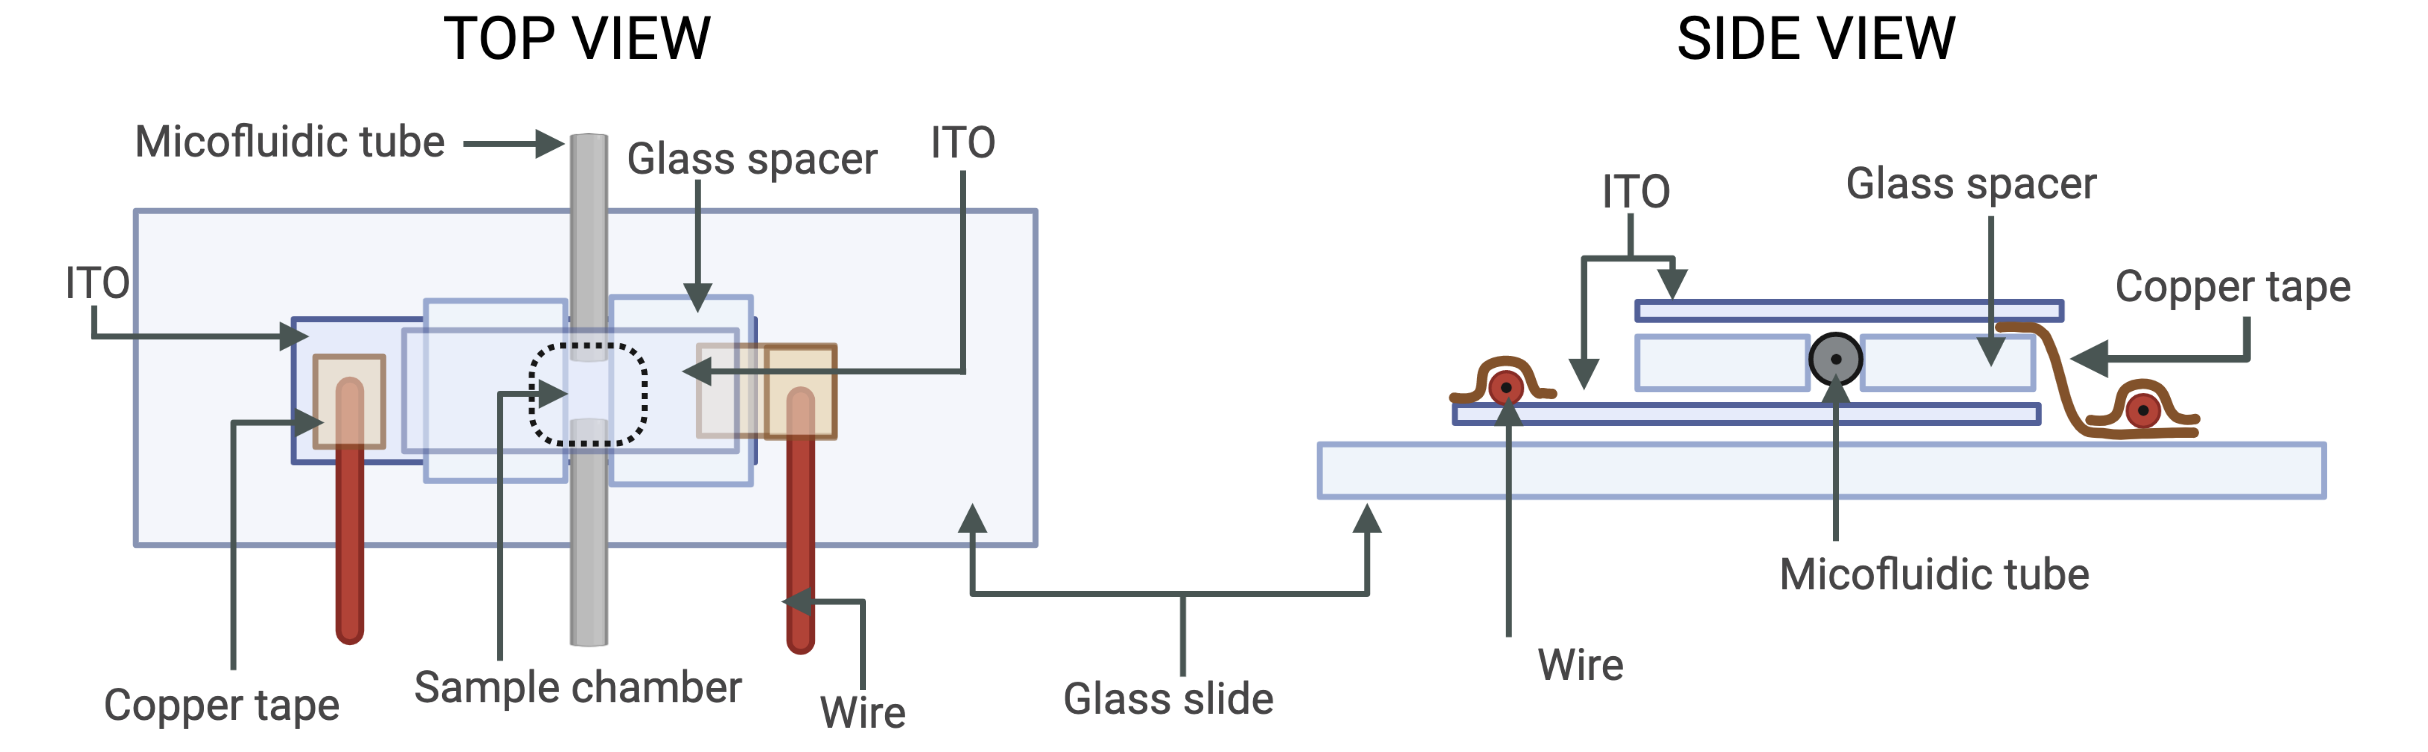
\includegraphics[width=\linewidth]{figsExpSystem/figSampleCell}
	\caption[Schematic representation of the sample cell.]{Schematic representation of the sample cell. The location where the gel and Janus particles will be located is labeled as the sample chamber. The cell is assembled from the bottom up, further details are provided in the section \ref{section:SampleCell}.}
	\label{fig:SampleCell}
\end{figure*}

Before the cell is assembled, the ITO must be coated with a thin layer of silica. Without this, the Janus particles will accumulate on the ITO surface due to the strong surface charge.
%\cite{kilic2011}
The silica layer acts to screen some of this charge so that the Janus particles remain dispersed throughout the gel. For the silica coating we use plasma enhanced chemical vapour deposition (PECVD): the ITO is run in the PECVD for 13 seconds at 300$^{\circ}$C as SiO$_2$ is deposited to form a layer of thickness 30nm. Importantly, approximately 1/3 of the ITO slide must be covered during the deposition of SiO$_2$, as a section must be kept clean for the electrical contact. 

Assembly of the sample cell proceeds from the bottom up and is constructed as follows:

\begin{enumerate}[label=(\roman*)]
	\item A glass microscopy slide forms the base (thickness 1mm). Upon this the first slide of ITO is glued with \textit{Norland 81} UV-curing glue, such that the ITO coated side is pointing upwards. Care is taken to note which end of the ITO is not coated in silica as this must be kept clear for the contact.
	\item A glass slide is cut to form the spacers. It is cleaned with ethanol  and then glued atop the ITO such that uncut straight edges point inwards and are spaced apart to create a channel wide enough for the microfluidic tubing. 
	\item Copper tape is attached to the glass spacer that is on the opposite side of the cell to the lower ITO contact. A small quantity of conductive epoxy (\textit{circuitworks}) is applied atop the inner end of the tape.
	\item The upper ITO slide is glued on top of the two spacers and the tape, with the ITO coated side facing down into the cell. 
	\item The cell is now ready for the gel, which will be inserted via a pipette. With the gel in place, the two tubes are inserted and glued in place with first a layer of UV-curing glue (\textit{Norland 81}) and then a layer of epoxy glue (\textit{Gorilla glue}).
	\item The wires are connected to the ITO contacts with copper tape and held in place with epoxy glue. This step is done last, after the gel has been sintered and the Janus particles flown into the sample chamber. 
\end{enumerate}




\begin{figure*}
	\centering
	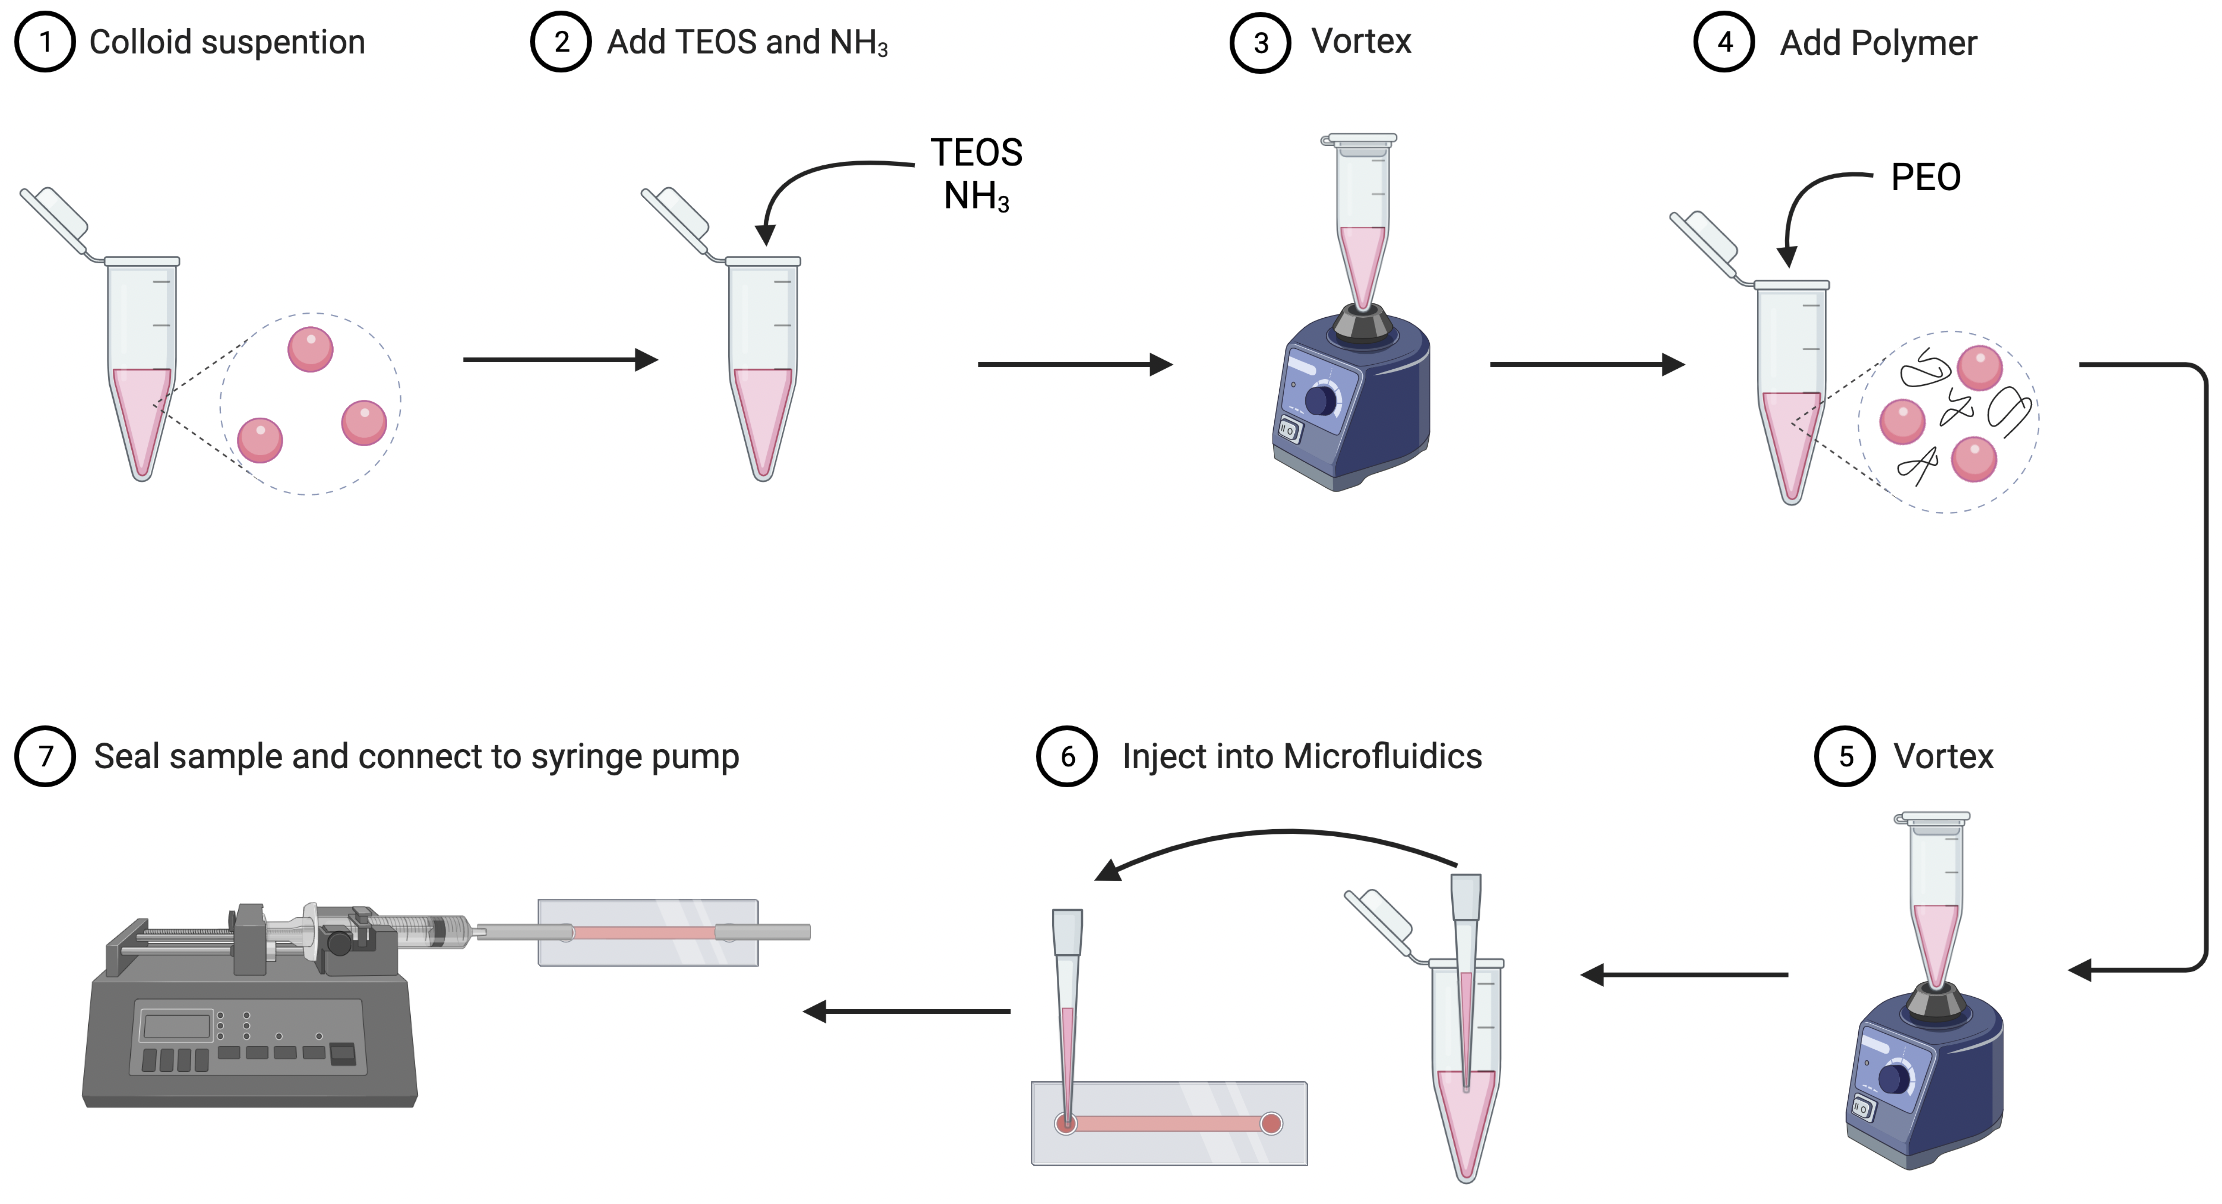
\includegraphics[width=\linewidth]{figsExpSystem/figFlowChart.png}
	\caption[Diagram for the preparation of a sintered colloidal gel within a microfluidic system.]{Illustrative diagram of the steps determined for the preparation of a sintered colloidal gel within a microfluidic system. These steps are further detailed in \ref{sec:AssemblyOfTheColloidalGel}.}
	\label{fig:FlowChart}
\end{figure*}


\subsection{Assembly of the colloidal gel}
\label{sec:AssemblyOfTheColloidalGel}


In the experimental system presented in this thesis, a colloidal gel serves as the complex environment within which the Janus particles undergo active dynamics. This colloidal gel is created through a self-assembly process driven by depletion interactions with non-adsorbing polymer depletants. However, this polymer must be removed before the Janus particles are added, as they would interfere with the activity and impose unwanted depletion forces upon the Janus particles. Before the polymer can be removed, an alternate mechanism to maintain the gel structure must be introduced. For this we grow a shell of silica around the gel network, sintering the particles together, after which the polymer can be removed. This process is undertaken with microfluidics, and therefore gel must be assembled within a microfluidic system, along with the reagents needed for the silica shell growth. In this section we detail process for assembling this system along with an accompanying schematic (Fig. \ref{fig:FlowChart}). The process is as follows:

\begin{enumerate}
	\item The fluorescent silica colloids are suspended in an eppendorf at a volume fraction of $\phi_c = 0.32$ in ethanol, where $\phi_c$ is the colloid volume fraction. This volume fraction is chosen to account for the volume of the silica growth reagents and the polymer-solvent solution to be added later. These further dilute the sample to a target colloid volume fraction  of $\phi_c \approx 0.2$, which is coherent with the model gel in Chapter \ref{chap:confinement}. This suspension is then mixed with a vortex for 30 seconds and then sonicated for 30 minutes to break up any aggregates. 


	\item The reagents for the growth of the silica shell via the Stöber process are added: tetraethyl orthosilicate (TEOS) is added at a concentration of [0.2M], and ammonium hydroxide (NH$_3$)  is added such that it is equal to 4\% of the solvent volume. These quantities match those of silica core-shell particle synthesis methods \cite{chen1996,chou2008,bogush1988}, aiming to grow a shell that is approximately 100nm thick.  
	\item The sample is mixed thoroughly with a vortex (15 seconds) to disperse the reagents homogeneously through the sample.
	\item The polymer is then added quickly to limit the amount of silica growth happening before the gel has formed. The polymer used for gelation is PolyEthylene Oxide (PEO) with a molecular weight: Mw = 5,000,000, and radius of gyration $R_G = 154$nm. For the silica colloids of diameter $\sigma$ = 850nm, this corresponds to a size ratio of $q = 2R_G/\sigma = 0.36$. 
	
		The PEO is dissolved in a 1:1 mixture of de-ionised water and ethanol at polymer concentration of $c_p=5$gL$^{-1}$. This mixture then added  via pipette such that the polymer volume fraction in the sample is $\phi_p \approx 4$, where assuming polymers are spheres of radius $R_G$:
	 
	 \begin{equation}
	 	\phi_{p}=\frac{V_{\mathrm{polymer}}}{V_{\mathrm{Total}}}=\frac{c_p N_{\mathrm{av}}}{M_W} \frac{4 \pi R_{G}^{3}}{3}
	 \end{equation}
	 
	 	where $N_{\mathrm{av}}$ is the Avogadro constant. 

	\item The sample is mixed thoroughly with a vortex (15 seconds) to disperse the polymer throughout the sample.
	\item A portion of the sample is injected into the sample cell (pre-assembled according to section \ref{section:SampleCell}) via pipette. This step must follow quickly on from step-5 as the large polymer volume fraction will cause the sample to undergo gelation rapidly, making it difficult to insert the sample into the narrow channel of the sample cell.
	\item With the sample in place, it must be connected to the microfluidics. The syringe pump is loaded with a 1mL volume syringe containing the solvent for imaging. This solvent must possess a matching refractive index to the silica colloids to reduce scattering during microscopy and produce the clearest images. Silica colloids have a refractive index of approximately 1.475$\pm 0.005$ at $\lambda$ = 500nm - 600nm, but this will vary slightly depending on the synthesis \cite{khlebtsov2008}. It is possible to match this index with a mixture of dimethyl sulfoxide (DMSO) and water, which have refractive indexes of 1.4768 and 1.333 respectively at $\lambda$ = 546nm \cite{lebel1962}.  
Through testing of several mixing ratios it was determined that a mixture of 10:2 for DMSO:water provided the best clarity for imaging. 

		Microfluidic tubing is attached to the end of the syringe with epoxy, and the pump is switched on until the tubing is filled with the solvent and any small bubbles removed. This tubing is then inserted into the channel of the sample cell. At the same time, another section of tubing is inserted into the opposing end of the channel to form the outlet. Both tubes are secured with first a layer of UV curing glue (\textit{Norland 63}) and then a layer of epoxy (\textit{Gorilla Glue}).	
\end{enumerate}



\subsection{Sintering the colloidal gel}

\begin{figure*}
	\centering
	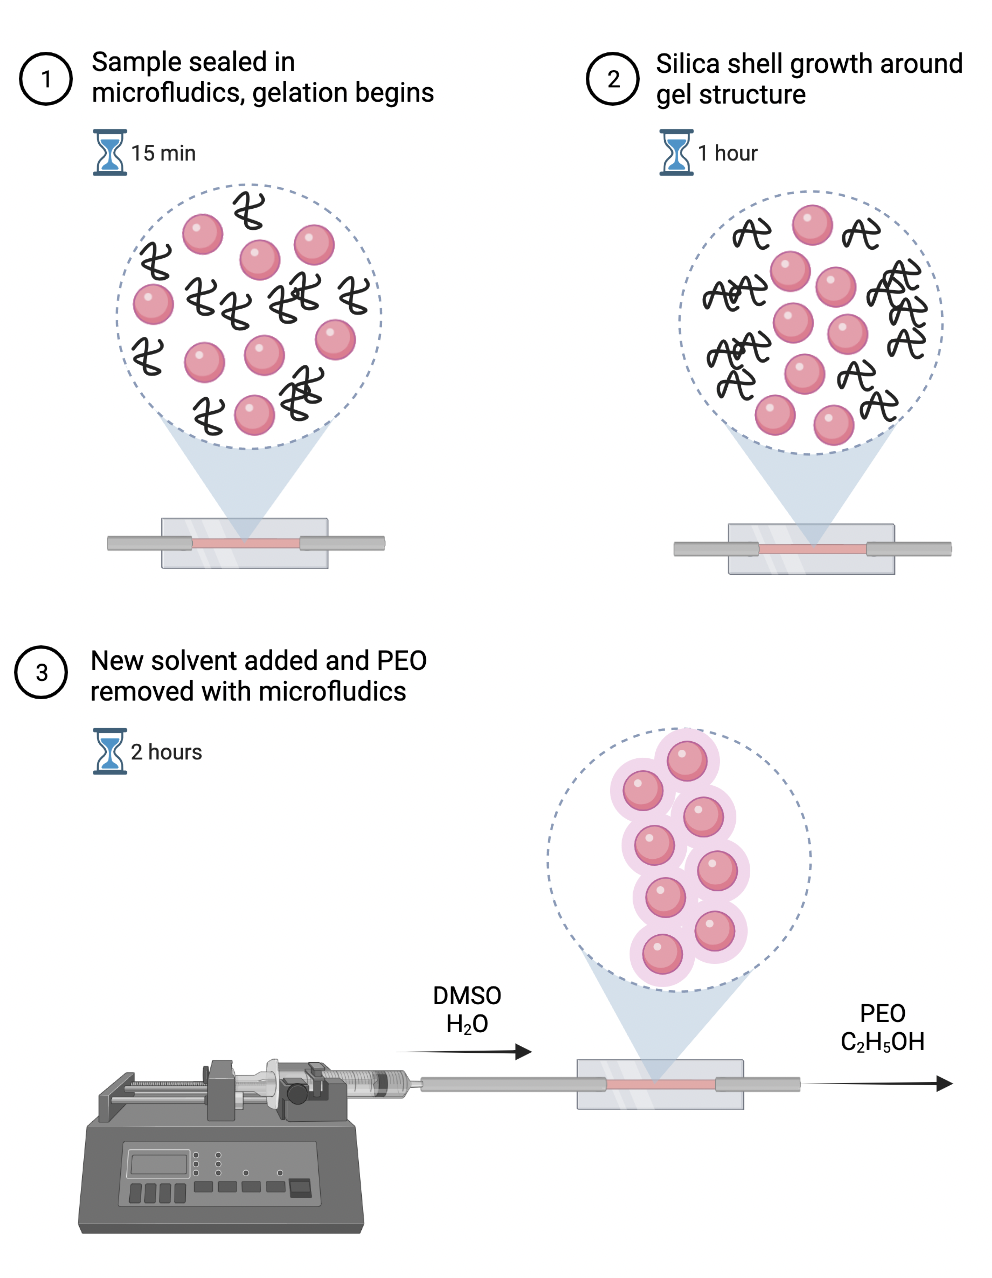
\includegraphics[width=0.8\linewidth]{figsExpSystem/figSintering.png}
	\caption[The gel sintering process]{The gel sintering process. Inset displays the microscopic structure at the beginning of each step. (1) The colloid polymer mixture begins the gelation process in the microfluidic channel. (2) When the reagents for the growth of silica are incorporated into the solvent: the silica colloids grow in close proximity; the areas of new growth overlap such that the gel network becomes a continuous silica structure. (3) With the gel sintered, the ethanol (C$_{2}$H$_{5}$OH) solvent containing the polymer (PEO) and any remaining silica growth reagents are rinsed out of the sample using the microfluidic syringe pump. A new solvent comprised of DMSO and water is flown in to replace it. }
	\label{fig:Sintering}
\end{figure*}

With the sample in place, the process for the sintering of the colloidal gel begins. This is the process through which the colloids will become physically joined together by the growth of the silica shell. This silica shell supersedes the polymer as the structural foundation of the gel network, making it possible to remove the polymer without destroying the branching colloidal structure. This process is carried out with microfluidics, the steps for which are depicted in Fig. \ref{fig:Sintering}, and proceed as follows:

 \textit{Step 1 ---} Within the sample chamber, the colloidal gel self-assembles as a result of the depletion interaction induced by the addition of the non-adsorbing polymer. The initial assembly happens relatively quickly ($\sim$15 minutes) as the colloids are arranged into the branching network structure. Over time this network will slowly coarsen as the particles rearrange causing the thickness of the branches to increase. 
 
\textit{Step 2 ---} The beginning of the silica growth happens in tandem with the gelation process. As soon as the TEOS and NH$_3$ are added to the solvent containing ethanol and water the Stöber process begins. In the early stages of this process, the gel network may not yet be fully established as newly synthesised silica begins to condense on to the surface of the silica colloids. As the gel comes together, this condensation process continues. However, at this point the colloids are held in close proximity by the polymer, and thus this new silica grows to bridge the gap between the particles. Over the course of an hour, this new growth of silica will create a shell around and throughout the gel network, creating a continuous silica structure strong enough to remain in place without the need for the polymer. 
	
	It must be noted, that while efforts are made to promote the rate of silica consumption (shell growth) and reduce the rate of regeneration (secondary nucleation) there may still be some secondary nucleation of new silica particles. These will not fluoresce like the original colloids and so will be invisible under the confocal microscope. However, as the secondary nuclei will be much smaller than the original colloids, the rate of sedimentation will be low \cite{royall2007}, and it is likely that they will be removed from the sample during the microfluidic transport in the following step.
	
\textit{Step 3 ---} After one hour, the sample will have undergone gelation due to the polymer and will have become sintered through the Stöber process. The colloidal gel network will now be stable independent of the polymer and so the polymer can be removed. The polymer is dissolved throughout the solvent surrounding the colloidal gel, its removal is carried out using microfluidics such that the original polymer-containing solvent is supplanted with a new polymer-free solvent. The original solvent is predominantly ethanol, with a smaller proportion made up of water, TEOS and NH$_3$, as well as the polymer PEO dissolved throughout.  This mixture is essential for the sintering process, but it is not suitable for imaging microscopy. The issue is that the refractive index of this solvent does not match that of the silica colloids, and as a result, light entering the sample is scattered causing the sample to look opaque. Therefore, the replacement solvent is a DMSO-water mixture, which provides a good refractive index match and is mounted in the syringe pump microfluidic system (according to step-7 in the previous section).

With the gel sintered, it is time for the DMSO-water solvent to be pushed through the sample using the syringe pump. Regarding the operation of the syringe pump, it is must be noted that the sample chamber is very small and cannot handle much pressure, and so the flow-rate must be kept low at 0.2$\mu$L/min for the first hour. The successful switching of these solvents will become evident through a change in the opacity of the sample; as the new solvent is introduced the refractive indexes of the colloids and the solvent will converge and the sample will become transparent. In addition to the index matching properties of the DSMO-water solvent, this solvent has the advantage that it is not soluble to the polymer PEO, further aiding to the removal of the PEO. Once it is clear that the new solvent has been incorporated, it is possible to increase the flow-rate up to  0.5$\mu$L/min, this is maintained for a further hour before the syringe pump is stopped. 




\subsection{Adding Janus particles to the sample}

%At this point the sample cell will contain a sintered colloidal gel surrounded by an index matched solvent. 
%For the addition of the janus particles, there are two considerations to be made: First, the janus particles are dense and sediment quickly (\fergus{as they are comprised of silica}); and second, the gel network while sintered is still fragile. It is for the consideration of the rapid sedimentation that the janus particles are not suspended within the DMSO:water solvent used in the solvent switching process. If that were the case, the janus particles would sediment in the syringe during the time it would take for the gel network to sinter and for the polymer to be removed. Then when the contents of the syringe would be infused into the sample, the janus particles would become stuck in the syringe.

\begin{figure*}
	\centering
	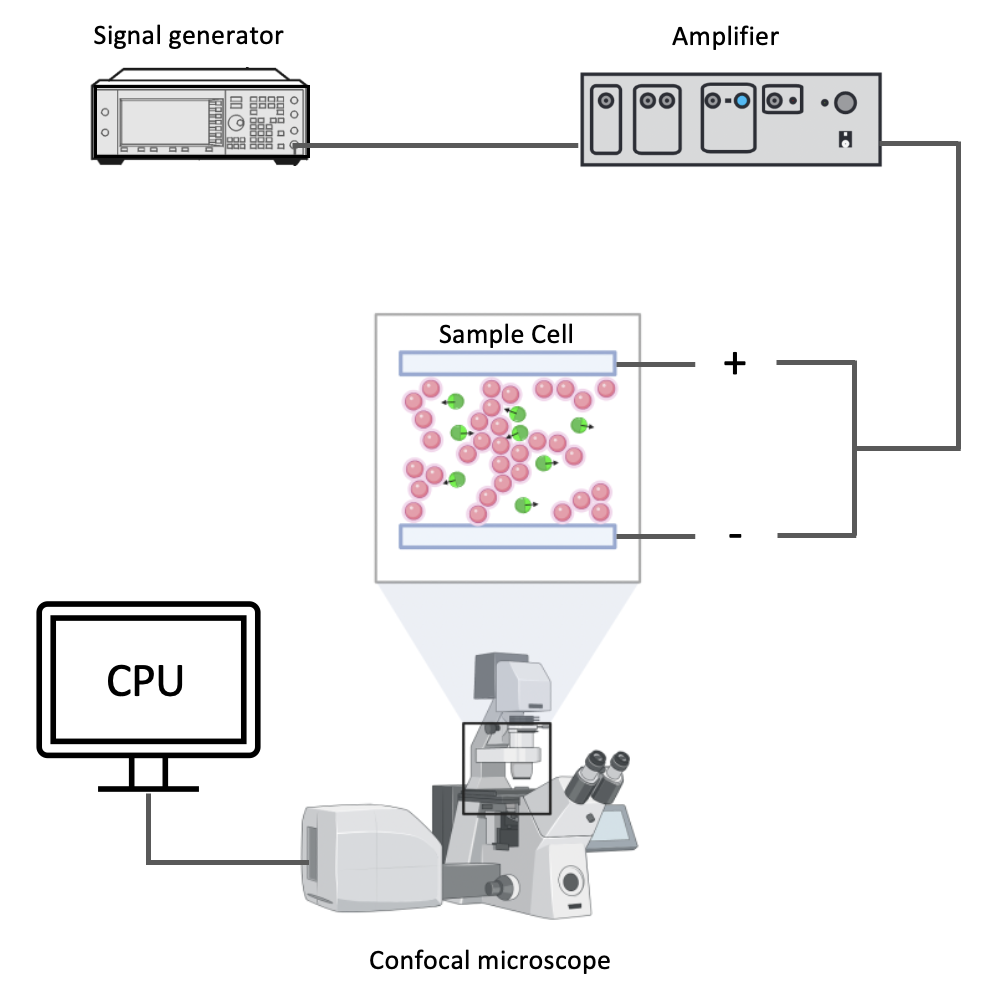
\includegraphics[width=0.7\linewidth]{figsExpSystem/figCircuit.png}
	\caption[Schematic for microscopy of the experimental system]{Schematic for the microscopy of the experimental system with the electric field.}
	\label{fig:Circuit}
\end{figure*}

Once the sintering process is complete, a suspension of  Janus particles is prepared in a DMSO-water solvent and drawn into a syringe which then loaded into the syringe pump. This new solvent mixture contains the same mixing ratio of DMSO:water, however there is an additional $10^{-4}\textrm{mol}/$L of salt (NaCl) included to screen charges between the Janus particles to prevent aggregation. As mentioned previously, the gel network is fragile and so when the syringes are exchanged in this microfluidic system, great care must be taken to avoid destroying the gel with large changes of pressure. Once the syringes have been exchanged, the Janus particles are flown into the gel at a rate of 0.5$\mu$L/min for 30 minutes to an hour, or until certain the Janus particle suspension has been incorporated into the sample. The timing is dependant on the length of the tubing between the syringe and the sample.

Once the suspension of Janus colloids has been incorporated into the gel, the microfluidic tubes are cut off and the ends sealed with epoxy. Finally, the wires are attached to the electrodes on the ITO with copper tape and held in place with more epoxy as in Fig. \ref{fig:SampleCell}. 


\subsection{Electric field}
With the sample preparation complete, the sample cell is mounted onto the microscope (\textit{Leica TCS SP8 confocal microscope}) and linked to the electrical circuit as shown in Fig. \ref{fig:Circuit}. The signal for the electric field is generated by a signal generator (\textit{Black star Jupiter 2010}) with a frequency of 5kHz. The signal amplitude is also set from the signal generator, however due to the relatively large distance between the electrodes an amplifier (\textit{Trek MODEL 609E-6}) is necessary to  reach voltages sufficient for Janus particle propulsion via ICEP in this sample cell. The sample cell is then connected to the amplifier.

When connected to the circuit, a uniform electric field is generated between the conductive ITO slides. The distance between the ITO slides is well-defined at 1mm by the glass spacers. The strength of this electric field $E = V / d$, where $V$ is the peak-peak voltage and $d$=1mm. The sample is viewed in real-time via the confocal microscope and data is collected for a range of field strengths $E$, set by controlling the voltage from the signal generator.



\section{Results and discussion}
\label{section:expSystem:Results}
In this section, we present results and analysis from the microscopy imaging of the 3D active system; broken down into three sections. 
First, a proof of concept result demonstrating the successful addition of Janus particles into the pores surrounding a sintered colloidal gel. 
Second, preliminary results showing 3D active particle dynamics and interaction with the gel network. Finally, an example of the usefulness of particle tracking methods for this system, with an extraction of the 3D coordinates of a sintered gel which are then subject to structural analysis.


\subsection{Brownian Janus particles in a gel}

\begin{figure*}
	\centering
	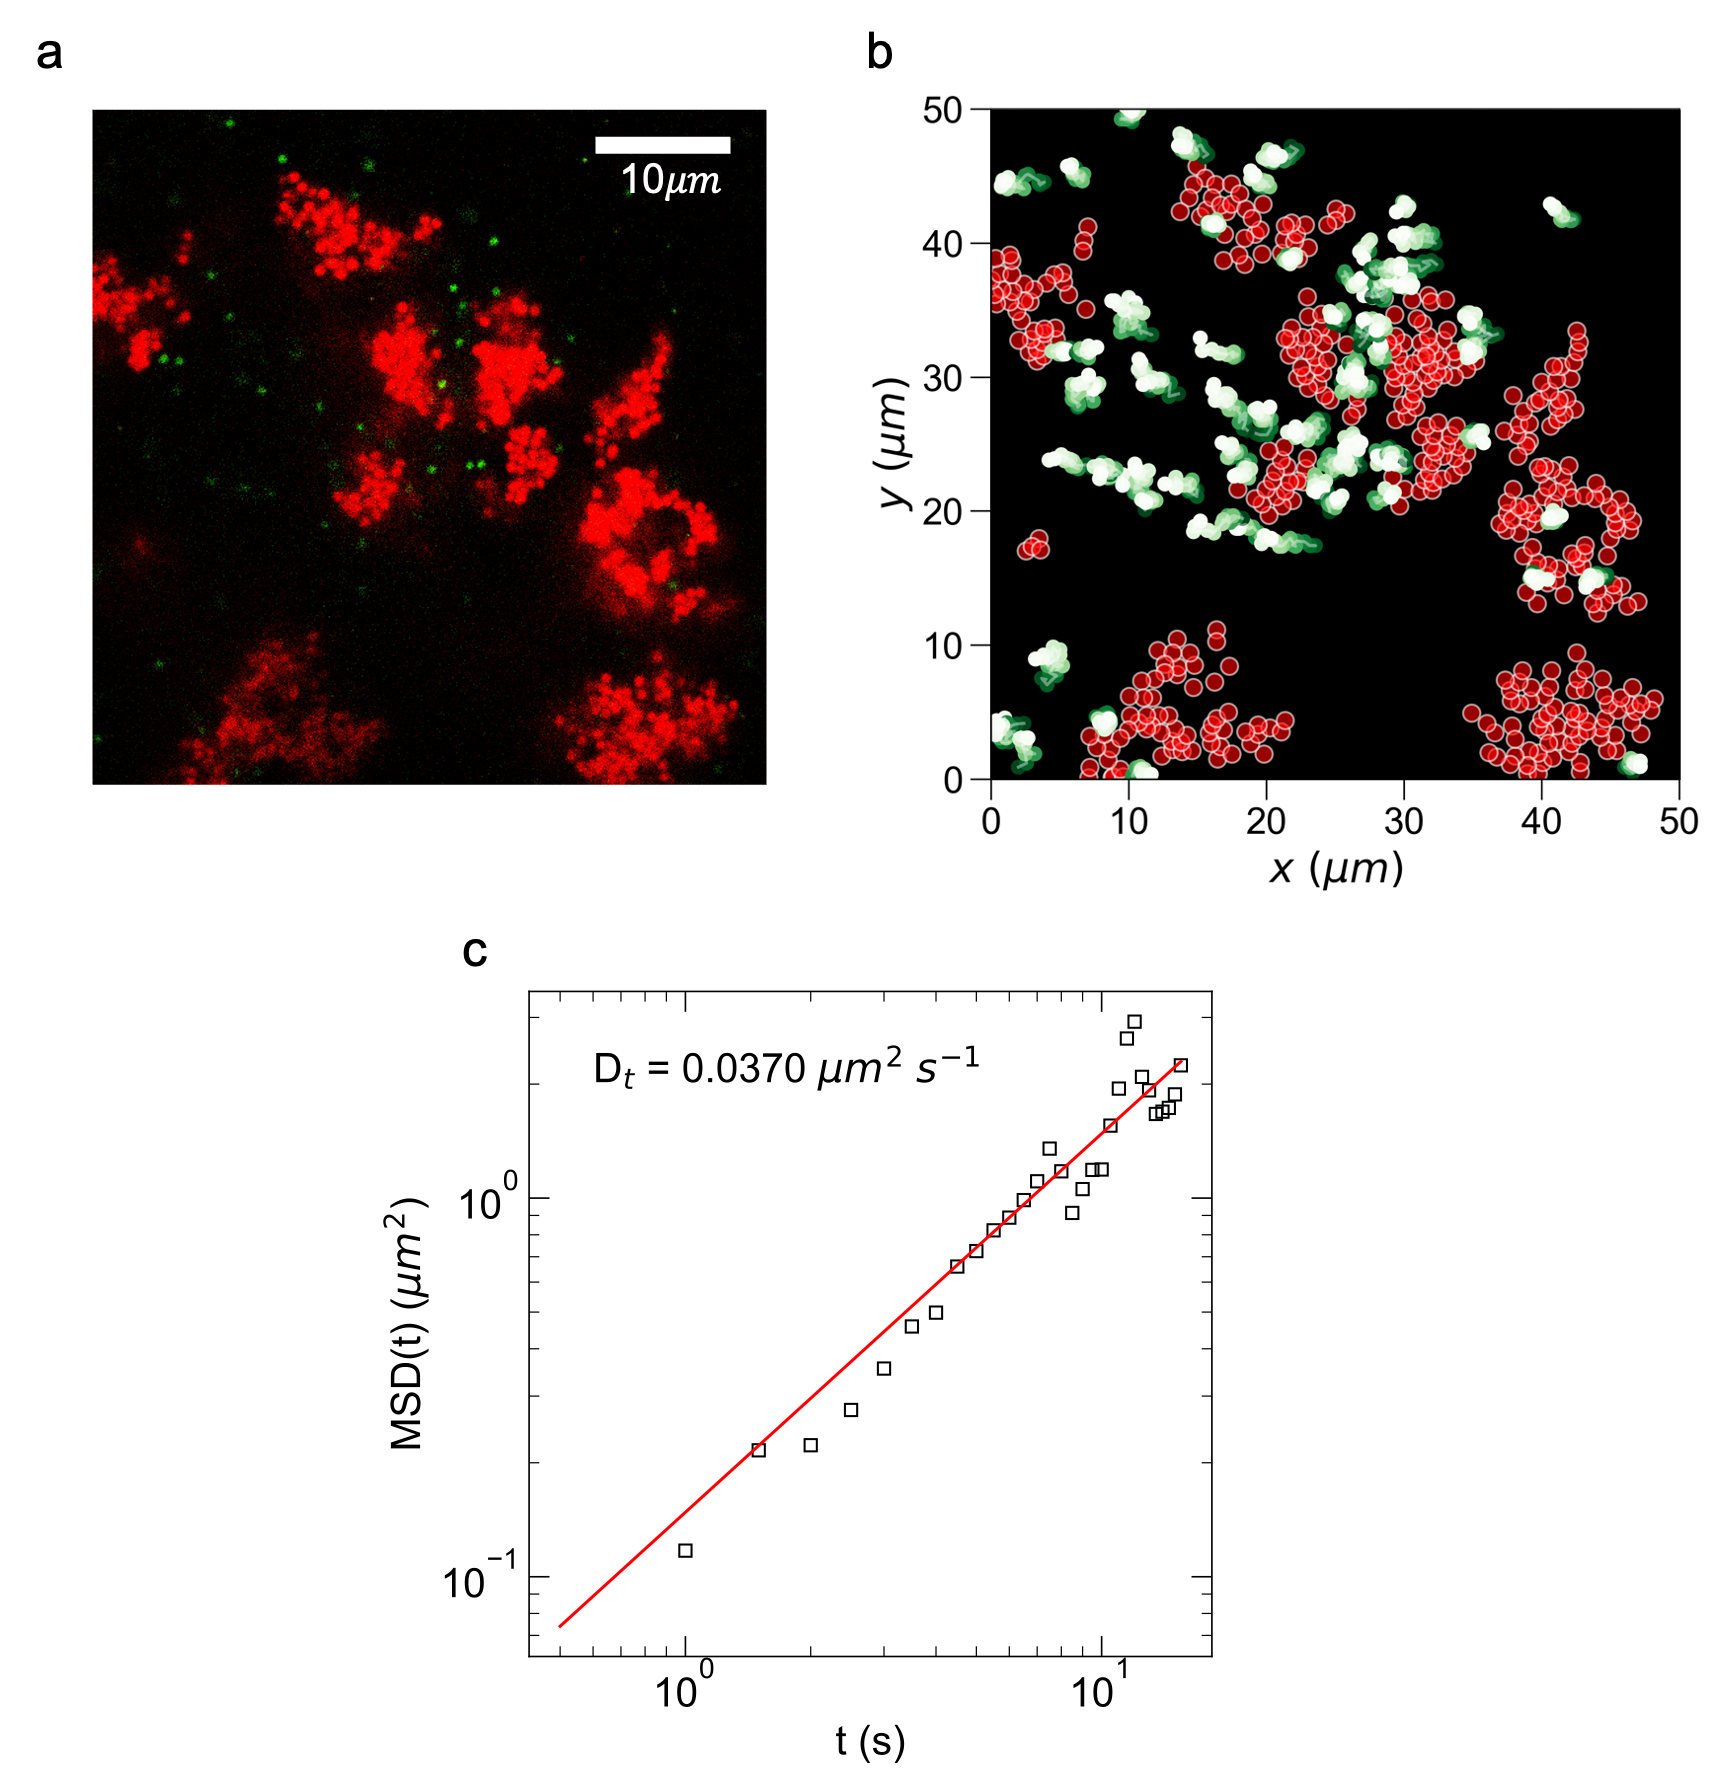
\includegraphics[width=\linewidth]{figsExpSystem/figBrownian}
	\caption[Brownian Janus particles in a gel]{\textbf{a} Confocal image of free Brownian Janus particles (green) dispersed through the voids surrounding a sintered colloidal gel (red). \textbf{b} Trajectories of tracked Brownian Janus particles within the sintered gel (red). Trajectories are coloured from green to white from the beginning to the end. \text{c} Mean-squared displacement of tracked Brownian Janus particle in a sintered gel. Fitting MSD = 4D$_t$t extracts a translational diffusion coefficient of $D_t = 0.037 \mu m s^{-1}$.}
	\label{fig:ExpPassive}
\end{figure*}


In the absence of the electric field, the Janus particles behave as Brownian colloids, a representative snapshot of this system is displayed in Fig. \ref{fig:ExpPassive}a. Here, we show a slice through the system obtained via confocal microscopy. There are two species of colloid in this image: the colloids belonging to the sintered gel (red) and the Janus particles (green). The particle types are imaged distinctly as a result of the two different fluorescent dyes incorporated throughout their particle centres; as a consequence, the gel colloids and the Janus particles fluoresce at different wavelengths and are thus measured independently by the microscope. This image shows that the Janus particles have successfully been injected into the pores of the gel network.

The image shown as Fig. \ref{fig:ExpPassive}a is taken from a series of images captured of particles in this slice evolving over time. In Fig. \ref{fig:ExpPassive}b we show trajectories of Janus particles in this slice over a 20 second period. Particle positions are tracked manually with \textit{Fiji} and then the coordinates are connected into trajectories with \textit{trackpy}. The gel particles are rendered in red, and the Janus particle trajectories are coloured from green to white corresponding to the beginning and the end of the measured trajectories respectively. Visual examination of these trajectories suggests that there is no clear directional bias; a characteristic of Brownian motion. Furthermore, there seems to be a distribution in the local density, with some some particles in the wider pores while others are located close to the gel surface or in narrow channels.

We calculate the mean squared displacement (MSD) from these trajectories and present the results in Fig. \ref{fig:ExpPassive}c. Given that this is a slice through the 3D system we fit the theoretical two-dimensional MSD$(t)$ = $4D_t t$  where $D_t$ is the translational diffusion coefficient. From this fitting it is possible to extract $D_t$, which in this case is measured to be 0.037$\mu$m$^2$s$^{-1}$. We compare this with the prediction from the Stokes-Einstein equation:

\begin{equation}
	D_t = \frac{k_B T}{6 \pi \eta r}
	\label{eq:StokesEinstein}
\end{equation} 

\noindent where $k_B$ is the Boltzmann constant, $T$ is the temperature assume to be 298K, $\eta$ is the dynamic viscosity which for this mixture of DMSO and water is 3.6cP \cite{catalan2001}, and r = 0.75$\mu$m corresponding to the radius of the Janus particles. These quantities predict a diffusion coefficient of $D_t$ = 0.0804$\mu$m$^2$s$^{-1}$. It is expected that this value should be greater than the measured value; eq. \ref{eq:StokesEinstein} describes the diffusion of a particle in an unbounded solvent, and thus does not consider the confinement effects imposed by the gel. 

In addition, given the dynamical nature of this system, a video of this data is available in the appendix (\ref{app:brownian}).


\subsection{Active Janus particles in a gel}
\begin{figure*}
	\centering
	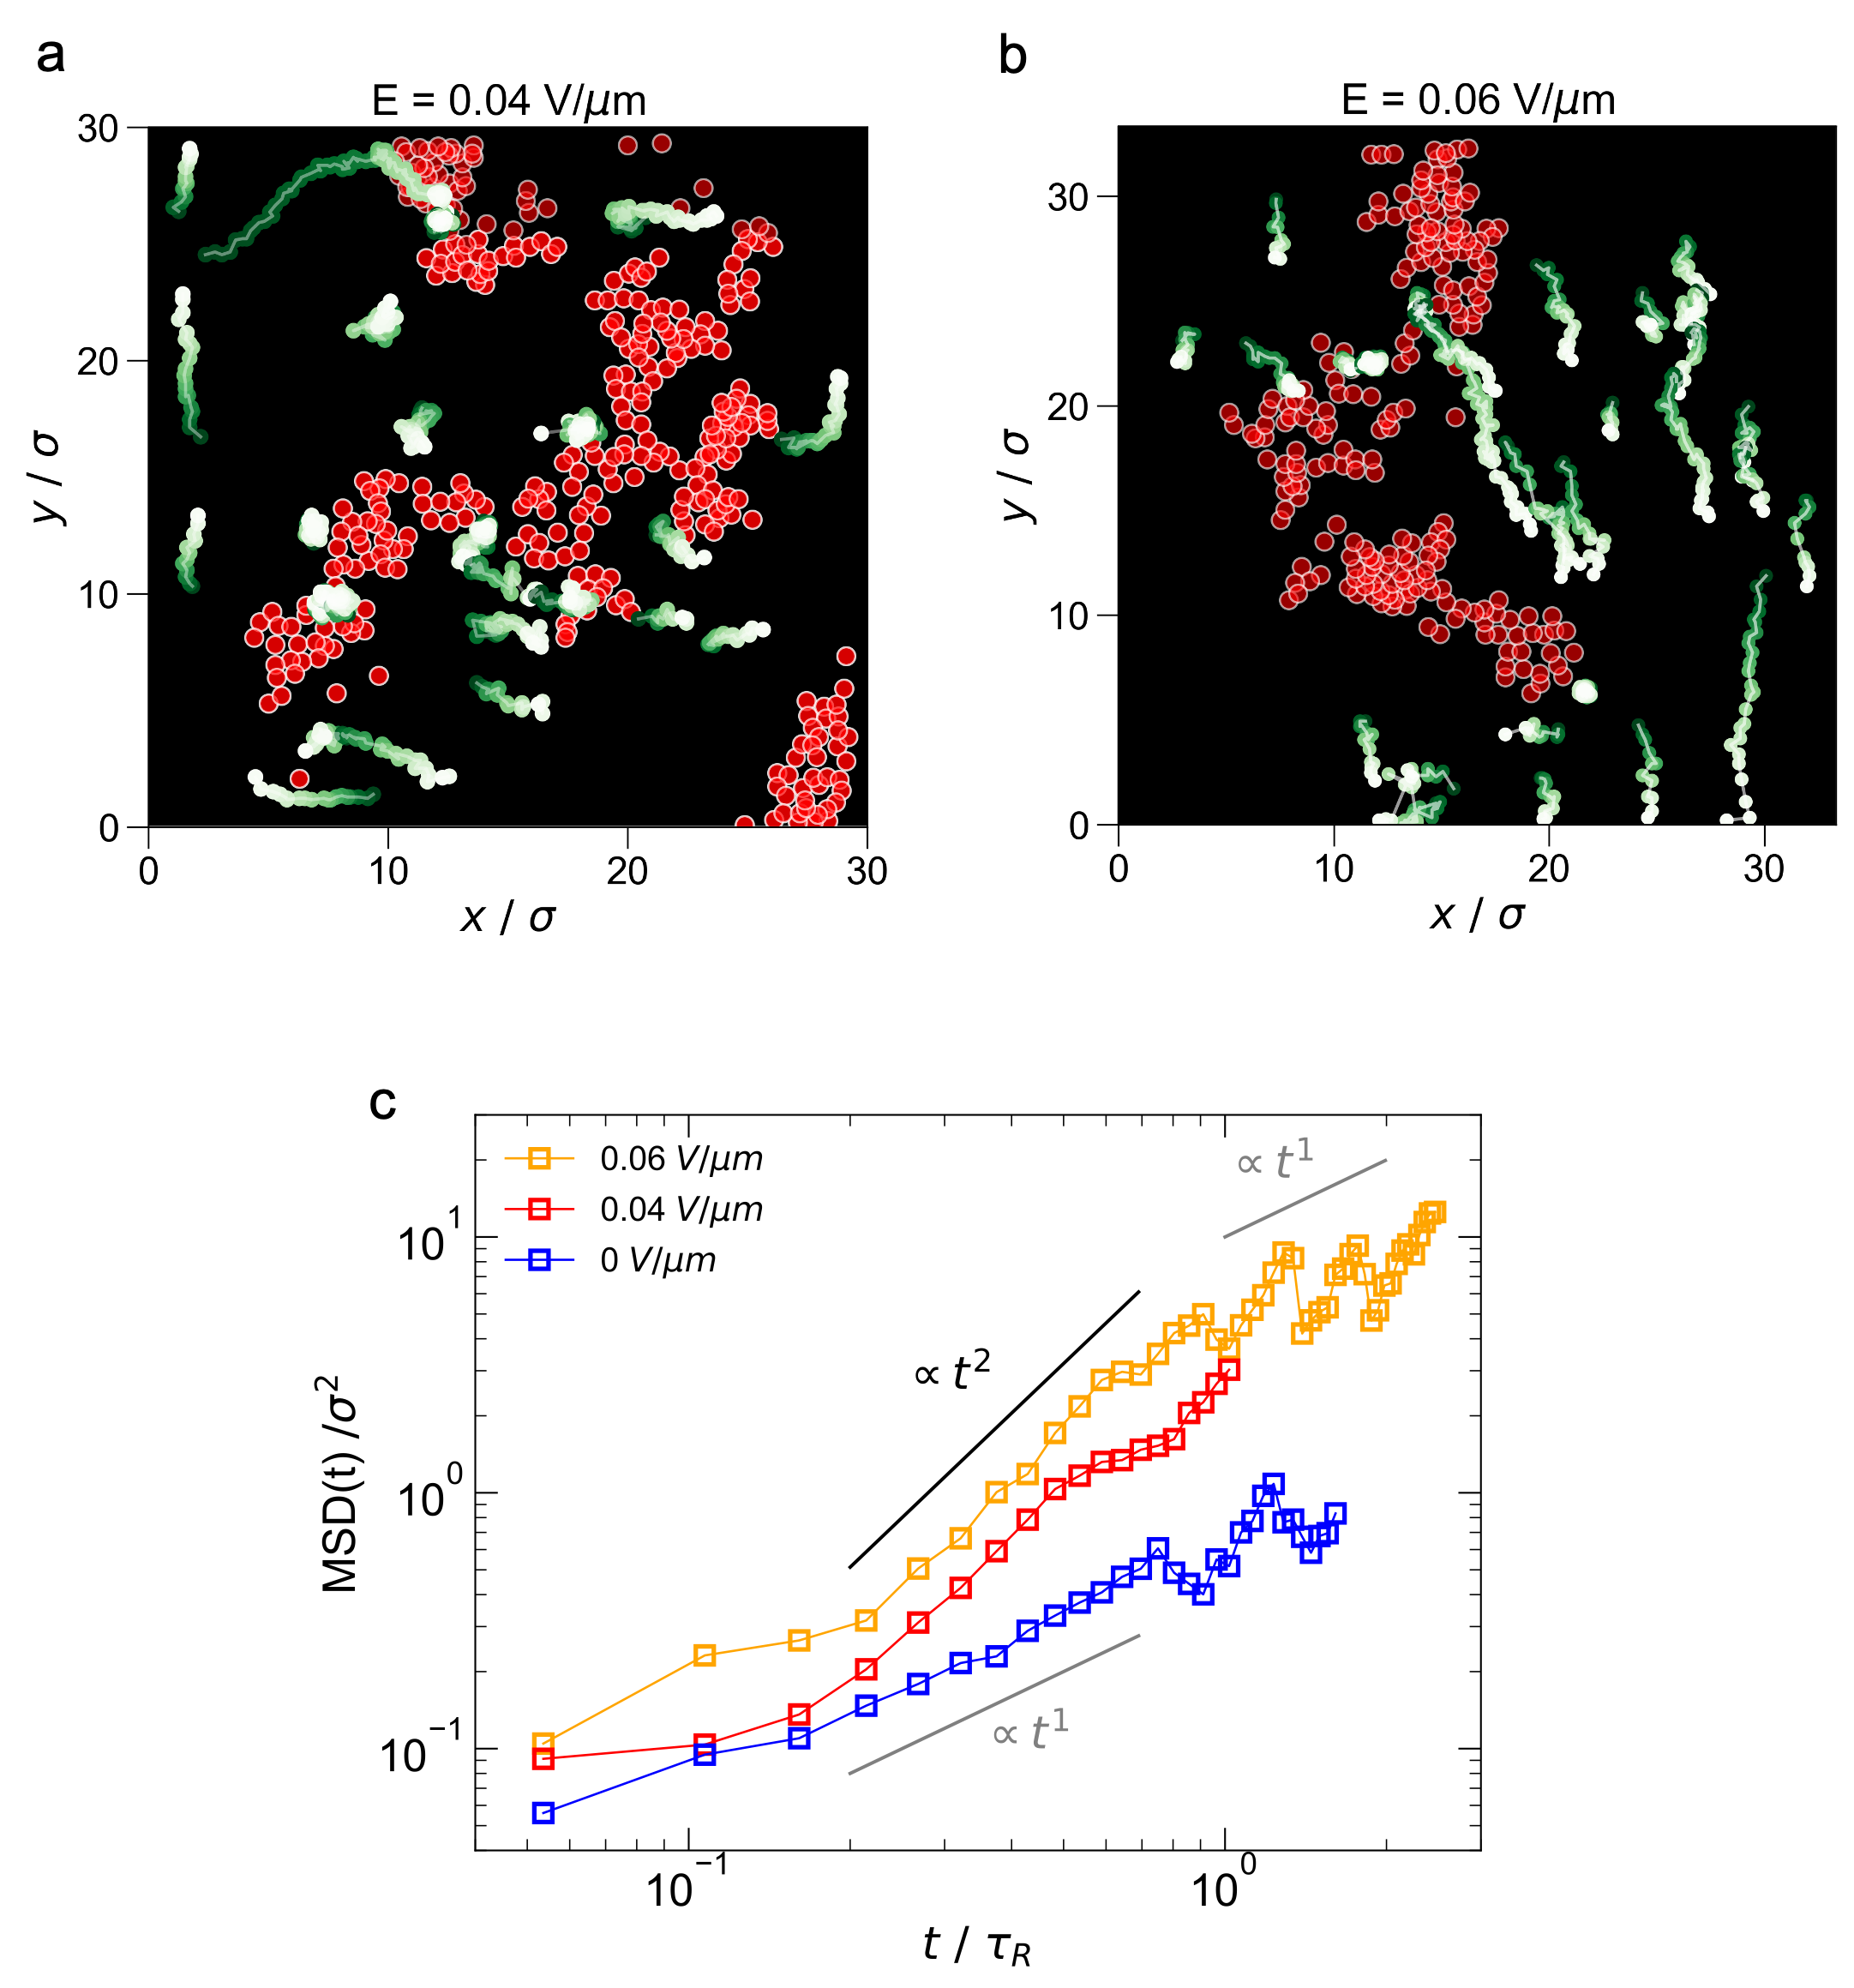
\includegraphics[width=\linewidth]{figsExpSystem/figJanusActive.png}
	\caption[Active Janus particles in a gel]{\textbf{a} Trajectories of tracked active Janus particles within the sintered gel (red) in an external field of $E = 0.04V/\mu m$. Trajectories are coloured from green to white from the beginning to the end. \textbf{b} as for in \textit{a} but with a field strength of $E = 0.06 V/\mu m$. \textbf{c} The mean squared displacement measure form the trajectories of Janus particles within the colloidal gel a three field strengths (0, 0.04, 0.06 $V/\mu m$), additional lines are plotted to help identify diffusive ($\propto t^1$) and ballistic ($\propto t^2$) regimes.}
	\label{fig:expActive}
\end{figure*}




In the presence of the external electric field, the Janus particles undergo active dynamics via induced-charge electrophoresis. Using the same methodology as was applied for tracking the passive dynamics, we extract trajectories from active Janus particles at two electric field strengths $E = 0.04 V/\mu$m and $E = 0.06 V/\mu$m, plotted in Fig. \ref{fig:expActive}a and Fig. \ref{fig:expActive}b respectively. Within these images the characteristic random and complex structure of the sintered gel is evidenced (depicted in red); as well as clear persistent motion in the active trajectories, displaying features that would not exist in an equilibrium system (depicted from green to white as a function of time). It should be noted that the trajectories in these figures are sourced from particles present in a slice through the 3D system, and therefore any out of plane dynamical information is lost.


Through examination of the trajectories at field strength $E = 0.04 V/\mu$m (Fig. \ref{fig:expActive}a), there are several notable features that can be highlighted. First, there appears to be a general trend that particles closer to the gel experience shorter in-plane displacements. This is most likely a result of trapping arising from the interplay of the persistent direction of propulsion and the complex gel surface structure. This is an effect that is expected to be significant given the findings in the model system presented in Chapter \ref{chap:confinement}; where the confinement of active particles could persist over several decades of the average rotational diffusion time.
Secondly, there is evidence of more transient interactions, where Janus particles encountering the surface of the gel translate laterally. This is a product of the particle's propulsion direction lying within an intermediate between directly into the gel and at an angle sufficient for escape. Finally, the velocities of active particles in this dataset seemingly bare no strong correlations with each other. A video of this data is available in the appendix (\ref{app:activejanus})
	
In Fig. \ref{fig:expActive}b, trajectories are extracted from Janus particles active in a field with an increased value of $E = 0.06 V/\mu$m. In this dataset, once again there is evidence of particle absorption at the gel surface, however, the most striking change at this higher field strength is the appearance of correlated particle motion. An observation of phenomenology such as this marks a necessary departure from the active Brownian model which does not consider alignment interactions. Given the propulsion mechanism of this system, these velocity correlations are likely as result of near-field hydrodynamic interactions. Similar phenomenology was observed by Nishiguchi \textit{et al.} \cite{nishiguchi2015}. in a system of ICEP Janus particles in 2D.
	
To compare the active dynamics at varying field strength we compute the mean square displacement and plot this in Fig. \ref{fig:expActive}c. The displacements are scaled by the diameter of the Janus particles $\sigma$. Furthermore, as with the translational diffusion coefficient in the previous section, it is possible to estimate the rotational diffusion coefficient $D_r$ via the Stokes-Einstein equation:

\begin{equation}
	D_R = \frac{k_B T}{8 \pi \eta r^3}
\end{equation}

\noindent which for this system yields $D_R = 0.107 \textrm{rad}/s$, and corresponds to a rotational diffusion time $\tau_R = 1 / D_R = 9.33s$. The time in Fig. \ref{fig:expActive}c is scaled by this $\tau_R$. 

As expected, with an increase in field strength the particles travel further on average, since the velocity of the propelling particles is proportional to square of the electric field strength \cite{gangwal2008}. In the previous section we established the liner scaling increase in the MSD in the case of passive particles, typical of diffusive Brownian dynamics. Here, in the presence of the field the Janus particles demonstrate a clear ballistic regime ($\propto t^2$) over the timescale of the rotational diffusion time $\tau_R$. Furthermore, at $E = 0.06 V/\mu m$ (for which the dataset covers a longer period of time), the particles move diffusively ($\propto t^1$) on average, at a higher effective diffusion over longer timescales. 


At higher electric field strengths ($E \approx 10^{-1} V / \mu m$), the field induces strong hydrodynamic flows in the solvent which overlap with active dynamics to an extent which is difficult to determine. This is behaviour that has not been seen in bulk systems and is likely a product of the larger sample cell size (a necessity for the inclusion of the microfluidics). At this field strength, the particles are accelerated to very high velocities such that it was not possible to extract particle trajectories, however this effect can be observed in a video provided in the appendix (\ref{app:janusHydrodynamics}).


\subsection{3D particle tracking of a sintered gel}
\label{sec:ParticleTracking}
\begin{figure*}
	\centering
	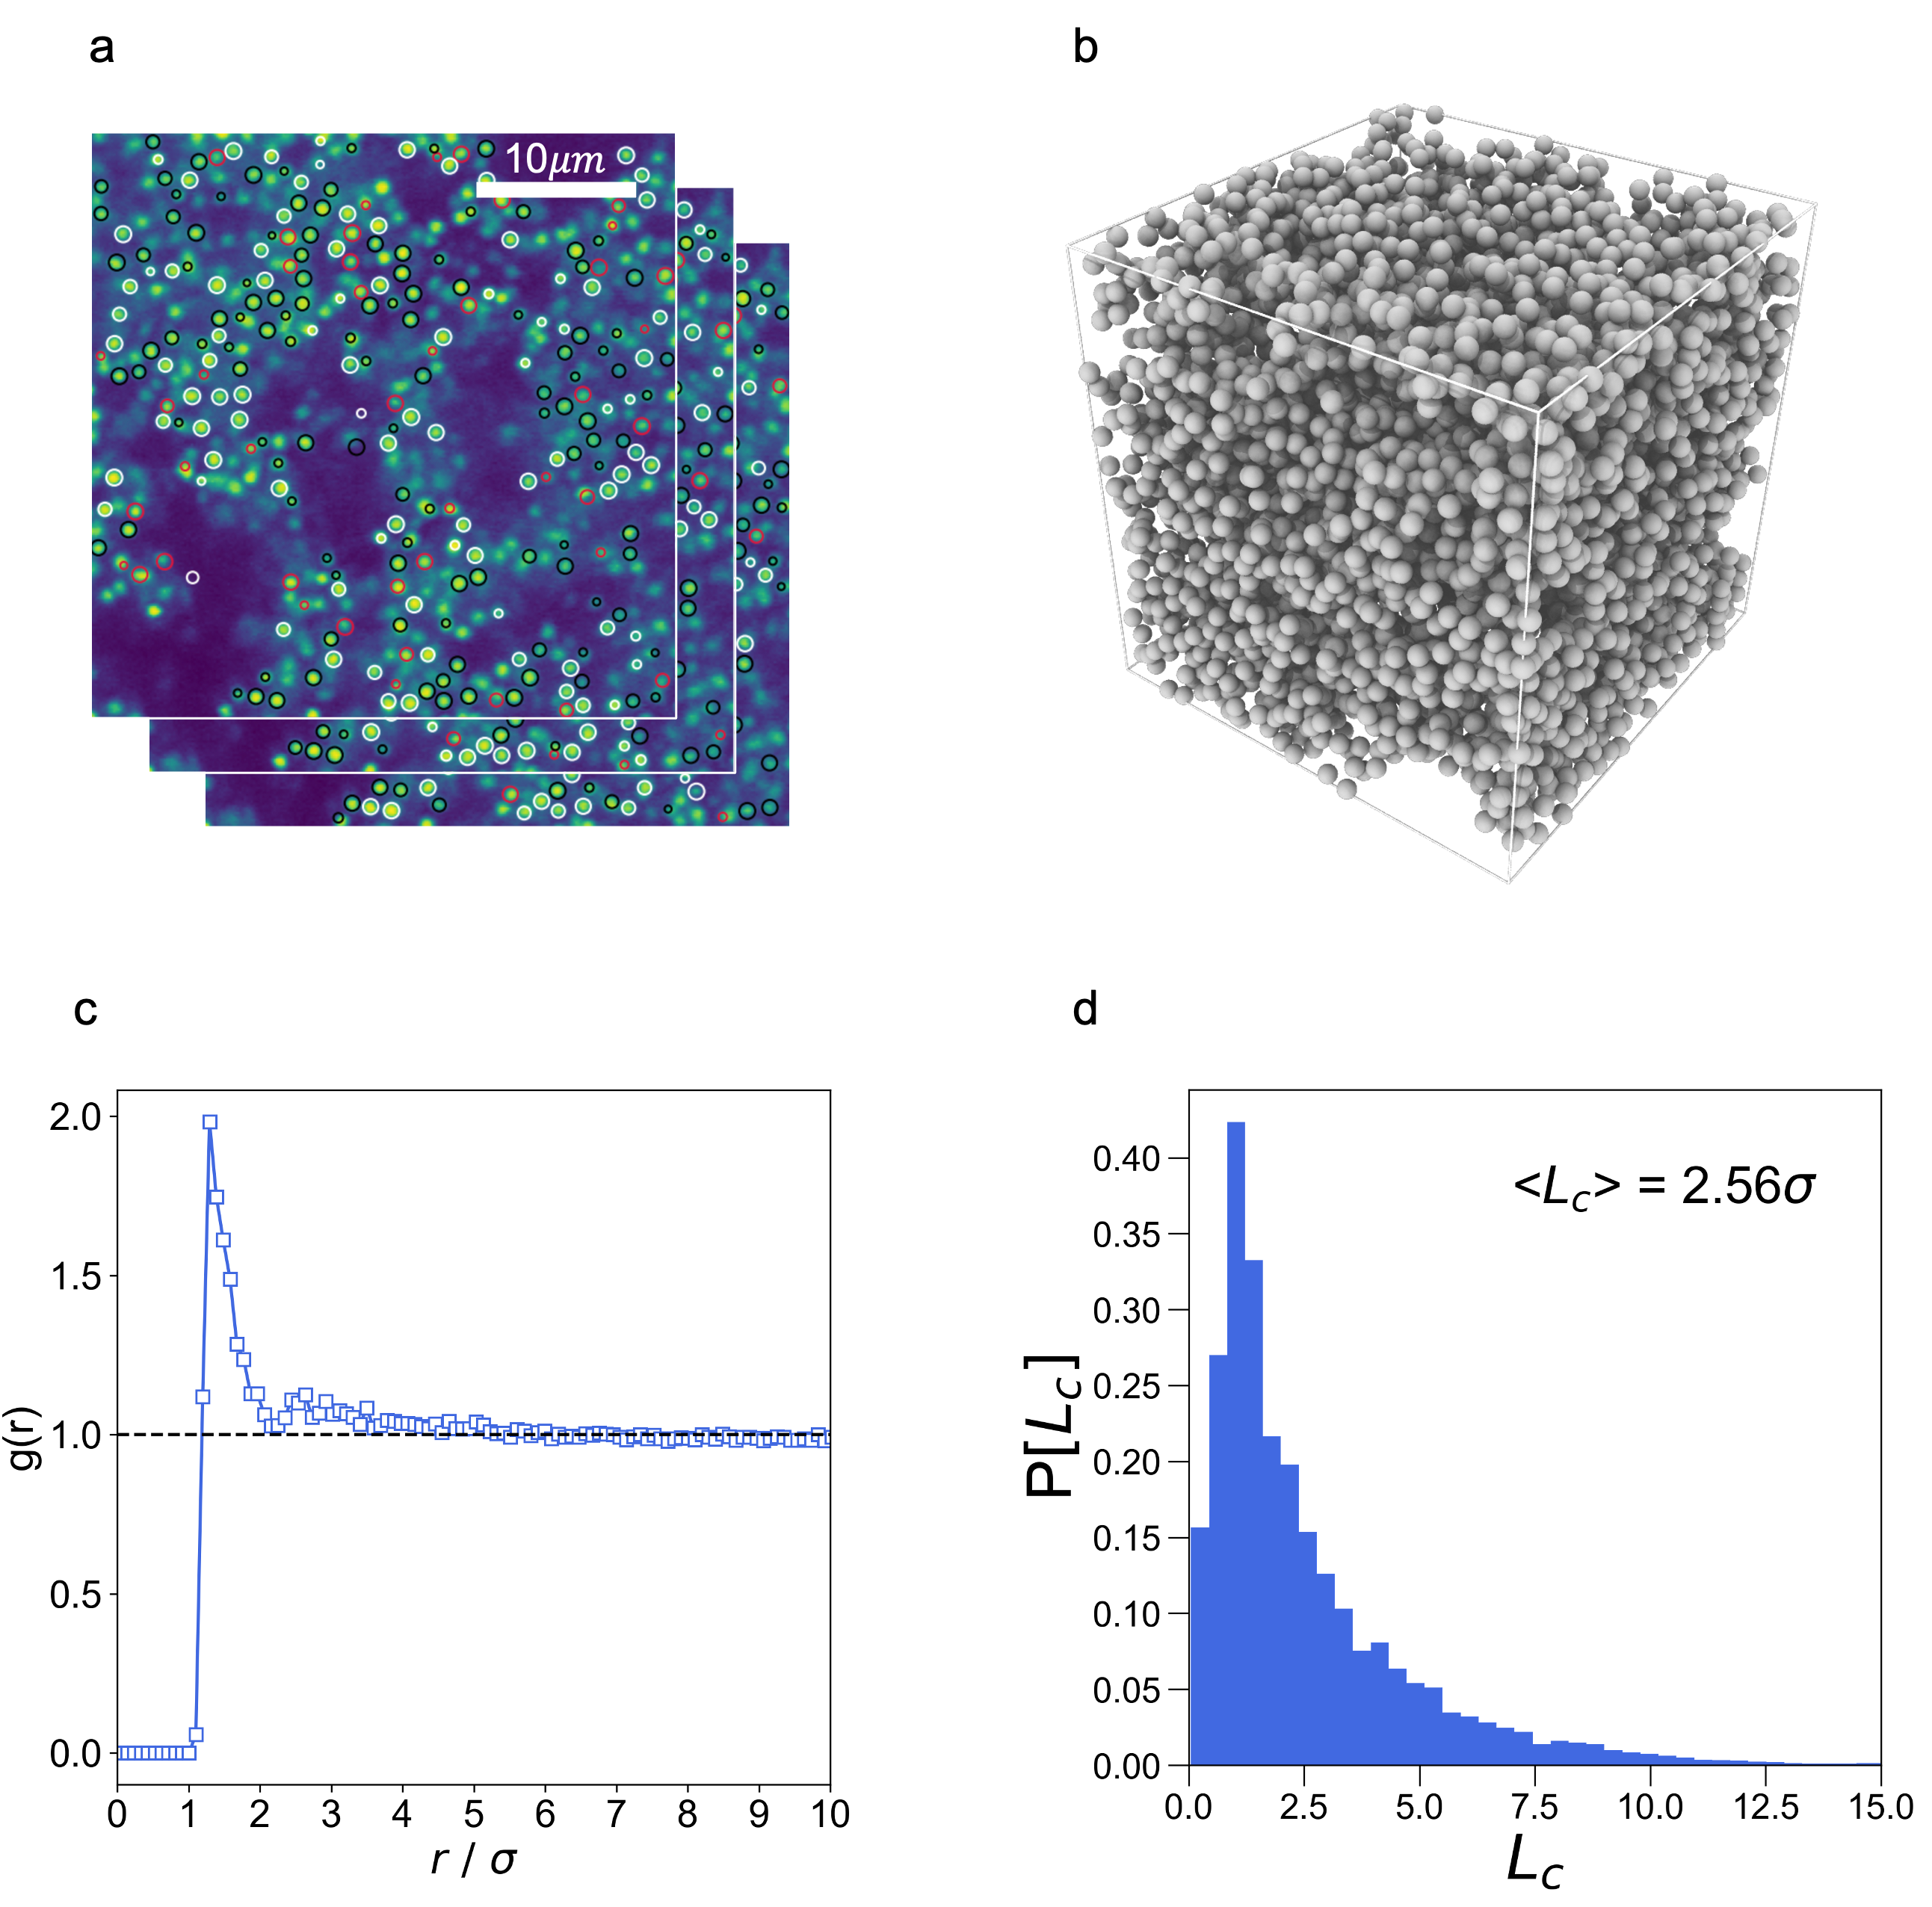
\includegraphics[width=\linewidth]{figsExpSystem/figParticleTracking.png}
	\caption[3D particle tracking of a sintered gel]{Particle tracking of a sintered colloidal gel. \textbf{a} Slices through the 3D gel with circles drawn marking particles that have been identified. Black and white circles are particles identified with \textit{trackpy} and the colour indicates whether the particle centres lie below or above the slice respectively. Red particles are identified using \textit{nplocate}. \textbf{b} A 3D rendering of the tracked gel coordinates. \textbf{c} The radial distribution function $g(r)$ for the tracked gel. \textbf{d} The pore chord length distribution measured from this gel sample.}
	\label{fig:ParticleTracking}
\end{figure*}


Thus far we have considered only information from the plane of activity of the Janus particles. Although the Janus particles are only diffusive in the plane parallel to the field, they interact with complex three-dimensional structure of the gel. Therefore, to truly understand the dynamics of this active system, it is necessary to have context for these dynamics in the form of structural information of the gel. This structural information is gained through the particle tracking methodology outlined in section \ref{section:expMethods:ParticleTracking}, an example of this method applied to confocal image data of a sintered gel is shown in Fig. \ref{fig:ParticleTracking}a. Here we see a stack of slices through the 3D gel, where the fluorescent colloids are seen to be arranged in the random branching network typical of a colloidal gel. Drawn on top of these images are circles representing particles that have been identified by the tracking algorithms, here the circle diameter indicates the distance of the particle centre from the image plane. 

From this information it is possible to recreate the 3D structure of the gel from the coordinates. The tracked co-ordinates are rendered in Fig. \ref{fig:ParticleTracking}b, showing the 3D structure of the gel and the voids around this network. Furthermore, from these 3D coordinates the radial distribution function $g(r)$ can be calculated, the result is plotted in Fig. \ref{fig:ParticleTracking}c. From this it is possible to determine the accuracy of the particle tracking; for hard spheres like these colloids there should be no correlation at distances less than the diameter and the distribution function should trend to unity at long distances. This is indeed what we observe in Fig. \ref{fig:ParticleTracking}c, indicating that a sufficient extraction of the 3D structural information has been achieved.

In addition, with these particle coordinates we measure pore chord length distribution using the same method as was used for the model gels in chapter \ref{chap:confinement}, the result is plotted in Fig. \ref{fig:ParticleTracking}d. From this information we can learn the lengthscale within which the Janus particles will be confined, for this sample the mean pore chord length for this gel was measured to be  $<L_c> = 2.56\sigma$.


\section{Conclusion and future Work}
\label{section:expSystem:Conclusion}


The work comprising this chapter has demonstrated the assembly of the first experimental observation of Janus colloids undergoing active dynamics in a 3D complex environment. The assembly of this system marks a major experimental development: being the first 3D active model in non-trivial confinement.

As a result of methodical experimentation, we have now established a detailed methodology for reproducing this system. One significant result arising from this work, is the successful supplanting of the gel assembly mechanism from the polymer induced depletion interaction, to a continuous silica shell; a result that could pave a way forward to further novel experimentation and analysis of porous heterogeneous systems. 
This development led to the primary result of this work, the observation of 3D active dynamics inside the gel. Active Janus particles within the gel network were observed exhibiting a range of interesting behaviours such as; transient accumulation at boundaries; trapping over long time scales in regions of high curvature; and an emergence of correlated particle velocities was observed, suggesting the presence of complex hydrodynamical interactions at higher field strengths. 
In addition to the analysis of the active dynamics, attention was paid to the structure of the gel network. Through particle tracking methods we are able to extract the three-dimensional coordinates from the microscopy images and use this information to conduct structural analysis of the gel network, providing context for the environment within which the active dynamics take place. 

This system holds great potential for new and exciting discoveries in this field. The work done so far has been significant in proving that such a system is possible within laboratory experiment. However, if further work were to be carried out it would be enlightening to do the following: 
First, it would be beneficial to map out the dynamical phase diagram at constant frequency: i.e. image the system at several densities and field strengths. 
This would give indications as to how dynamical phenomena manifest for active Janus particles in confinement when compared to the bulk. It would be especially interesting to observe the system with the Janus particles at high density and to investigate whether this system would phase separate in the same way as the model presented in chapter \ref{chap:confinement}.
Furthermore, if this system were imaged again; before recording planar active dynamics, it would be advantageous to scan the gel network in 3D, so that out-of-plane information would be available to provide context to any dynamic analysis. Even better would be to track the active dynamics in 3D. This would necessitate imaging at a lower resolution and with a greater magnification so that the 3D scanning is quick enough to capture the dynamics in the three-dimensions. 



One aspect that was not observed in this system and that was present in the bulk, is dipolar interactions. In the bulk systems, these interactions emerge at high field strengths. However in this system, it is likely that these are being interrupted by the large hydrodynamic flows that are present in this larger sample chamber. 
Therefore, if it were possible to downsize the design of this system such that these flows were reduced; it would be of interest to study the interplay between the active population of the Janus particles and the dipole interactions in the presence of the complex environment created by the gel. Specifically, it would interesting to see in which ways the elongated active dipolar strings are influenced by the gel structure, and whether the emergence of order introduced though dipole-dipole interactions persists.
Furthermore, since all of the dynamics of active particles in this work have resulted from ac fields at 5kHz, and studies of two-dimensional active colloids propelling through the same mechanism have been shown to exhibit striking behaviour at higher frequencies; it would be of interest to study this system at higher frequencies.

Finally, all of these suggested extensions could be compared a model system implemented using molecular dynamics, like that of chapter \ref{chap:confinement}. 




\section*{Acknowledgments}
	We would like to thank Katherine Skipper for carrying out the synthesis of the Janus particles used in this work, and Ioatzin Rios de Anda for many helpful discussions. The cartoon figures presented in this chapter were made with BioRender. 

